\newpage
\section{Text Mining}
%\begin{figure}[H]
%  \centering
%  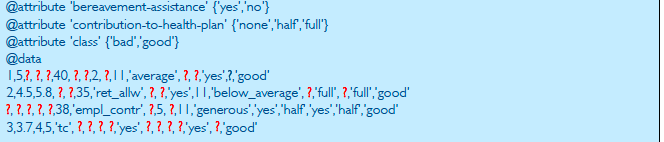
\includegraphics[width=.5\linewidth]{arffmissing}
%\end{figure}
Text mining deals with the discovery of \textbf{new} ,previously \textbf{unknown} ,\textbf{information} by extracting automatically information from different \textbf{unstructured textual documents}.\\
Text mining is used for:
\begin{itemize}
\item Classification
\item Clustering
\item Sentiment Analysis
\item Summarization
\item Relation/Concepts/Events extraction
\item Topic modelling
\item ...
\end{itemize}
The goal is to turn \textbf{text data} into high-quality information that :
\begin{itemize}
\item minimizes \textbf{human effort}
\item supplies \textbf{knowledge} for optimal decision making
\end{itemize}
Text mining is strongly related to \textbf{text retrieval} which is an essential part of the task.

\subsection{NLP}
Natural language processing is a very important field in text mining.
Natural language is designed for \textbf{efficient} human communication. This often results in \textbf{omitting} a lot of \textbf{common sense knowledge} which we assume the reader/hearer possesses and results also in a lot of \textbf{ambiguities} which we assume the reader/hearer know how to resolve.\\
This makes NLP very difficult for many reasons : 
\begin{itemize}
\item \textbf{Word-level ambiguity} : "design" can be noun or verb, "root" as many meanings...
\item \textbf{Syntactic ambiguity} : "a man saw a boy with a telescope"
\item \textbf{Presupposition} : "he has quit smoking" implies he smoked
\end{itemize}
An is as today still a field with many open problems.

\subsection{Information Retrieval}
Deals with the problem of locating \textbf{relevant documents} with respect to the \textbf{user input or preference} used for example in on-line library catalogs or document management systems.\\
Must deal with :
\begin{itemize}
\item Management of \textbf{unstructured documents}
\item Approximate search
\item Relevance
\end{itemize}

There are 2 modes of \textbf{text access}:
\begin{enumerate}
\item \textbf{Pull mode (Search Engine)}\\
The user takes initiative and gets ad-hoc information
\item \textbf{Push mode (Recommender Systems)}\\
The system takes initiative having good knowledge about a user's need.
\end{enumerate}

Then there are 2 steps in \textbf{text retrieval}:
\begin{enumerate}
\item \textbf{Document Selection}\\
This is \textbf{keyword-based } retrieval where a \textbf{query} defines a series of requisites and only documents that satisfy them are returned. \\E.g.: \textbf{Boolean Retrieval Method}
\item \textbf{Document Ranking}\\
This is \textbf{similarity-based} retireval where documents are ranked on basis of relevance wrt to the user query : for each document a  \textbf{degree or relevance} is computed wrt to the query.\\E.g.: \textbf{Vector Space Model}
\end{enumerate}

\begin{figure}[H]
  \centering
  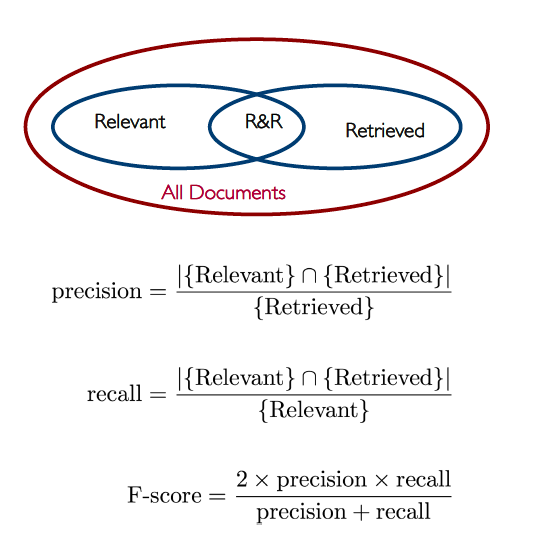
\includegraphics[width=.7\linewidth]{text1}
\end{figure}

A document and a query are represented as \textbf{vectors} in high-dimensional space corresponding to\textbf{ all the keywords}. \textbf{Relevance} is measured with an appropriate similarity measure defined over the vector space.
\\
How to select \textbf{keywords} to capture \textbf{basic concepts}?\\
How to assign weights to them?\\
How to measure similarity?\\

\begin{figure}[H]
  \centering
  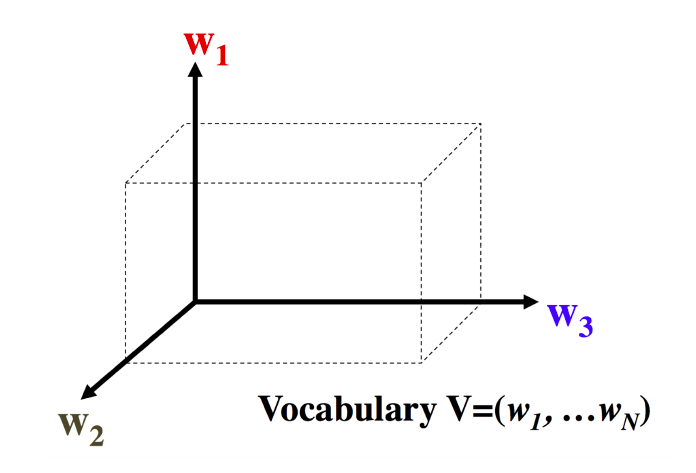
\includegraphics[width=.7\linewidth]{text2}
\end{figure}
In the figure an example with a 3 word vocabulary that creates a 3D space and below an example of document (bag of words does not consider \textbf{order}) and query inside such a space.
\begin{figure}[H]
  \centering
  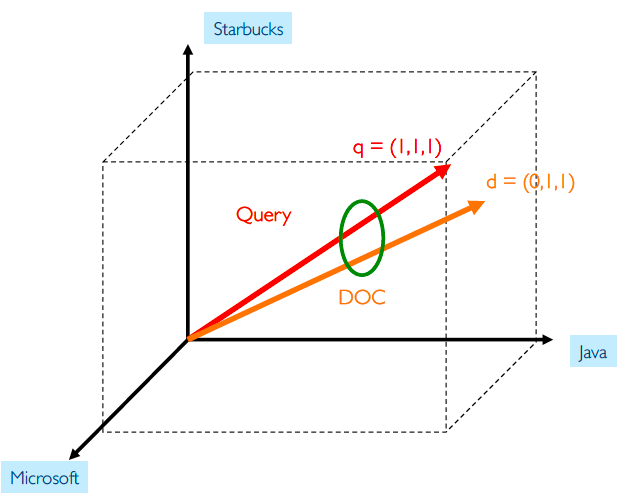
\includegraphics[width=.7\linewidth]{text3}
\end{figure}
The similarity is given by the \textbf{angle} that forms between the two vectors.\\

\subsection{Ranking Documents}
Given\begin{itemize}
\item a query $q=q_1,...,q_m$ where $q_i$ is a word 
\item a document $d=d_1,...,d_n$ where $d_i$ is a word (bag of words model)
\item \textbf{Ranking function} f(q,d) return a \textbf{real value}
\end{itemize} 
A \textbf{good} ranking function should put relevant documents over non-relevant documents.The key challenge is how to measure the \textbf{likelihood} that document d is relevant to query q :
\begin{itemize}
\item \textbf{Similarity-based models} : 
Uses the vector space model (our focus!)
$$ f(q,d) = similarity(q,d)$$ 

\item \textbf{Probabilistic models}:
Classic probabilistic models, language models or divergence from randomness models
$$ d(q,d) = p(R=1 |d,q)$$

\item \textbf{Probabilistic inference models}:
$$ f(q,d) = p(d \implies q)$$

\item \textbf{Axiomatic model}:
$f(q,d)$ must satisfy a series of constraints.
\end{itemize}

\subsubsection{1.Document Similarity Retrieval:VSM} 
A way to measure similarity between query and documents is using the dot product:
\begin{figure}[H]
  \centering
  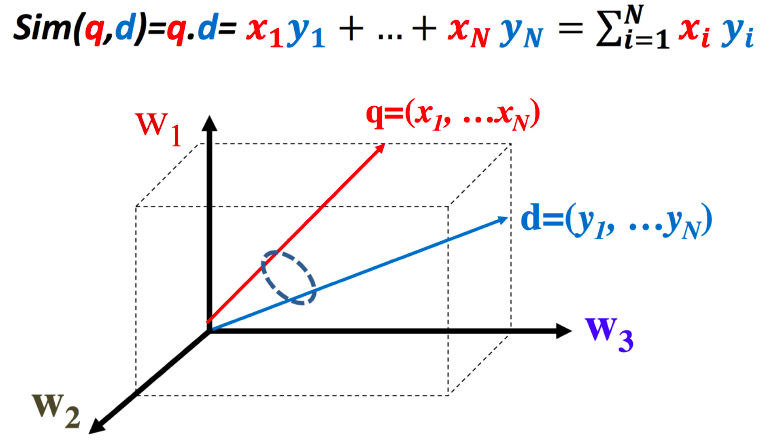
\includegraphics[width=.7\linewidth]{text4}
\end{figure}
Each word is either 0 or 1 depending on if it is found in the document/query or not:
\begin{figure}[H]
  \centering
  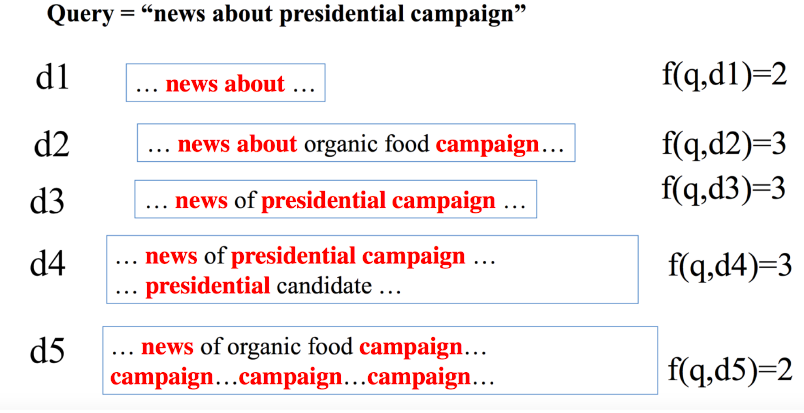
\includegraphics[width=.7\linewidth]{text5}
\end{figure}
This a \textbf{basic approach} which yields good results but can be improved : when searching for a query certain words are repeated more than once and deserve more credit or certain words have \textbf{bigger weight} than others (e.g.: presidential $>$ about)

\subsubsection{2.Document Similarity Retrieval : TFW}
A solution to weighting common words more is used \textbf{Term Frequency Weighting}:
\begin{figure}[H]
  \centering
  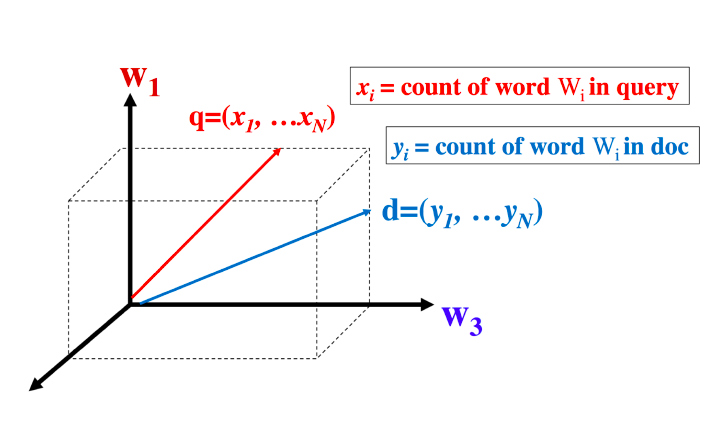
\includegraphics[width=.7\linewidth]{text6}
\end{figure}
\begin{figure}[H]
  \centering
  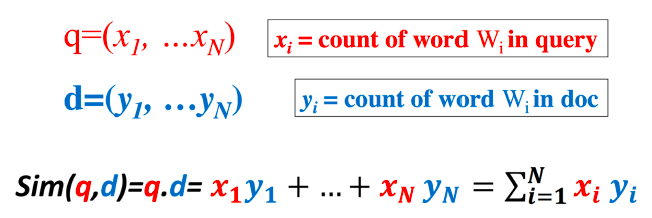
\includegraphics[width=.7\linewidth]{text7}
\end{figure}
An example :
\begin{figure}[H]
  \centering
  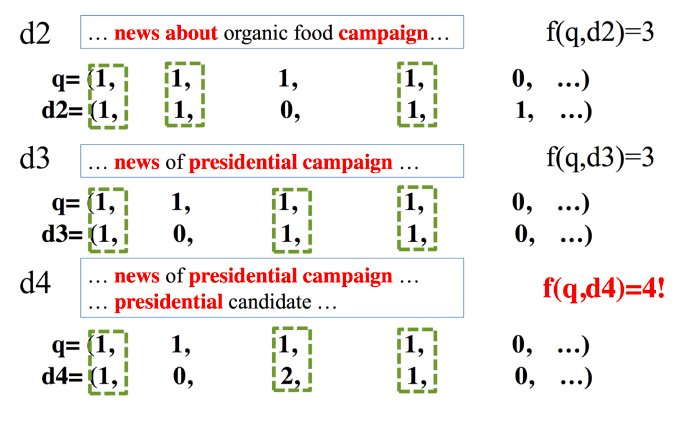
\includegraphics[width=.7\linewidth]{text8}
\end{figure}
This still does not solve that some words are more important than other ("presidential" $>$ "about")

\subsubsection{3.Document Similairty Retrieval : IDF}
TFW can be extended using the \textbf{Inverse Document Frequency} 
\begin{figure}[H]
  \centering
  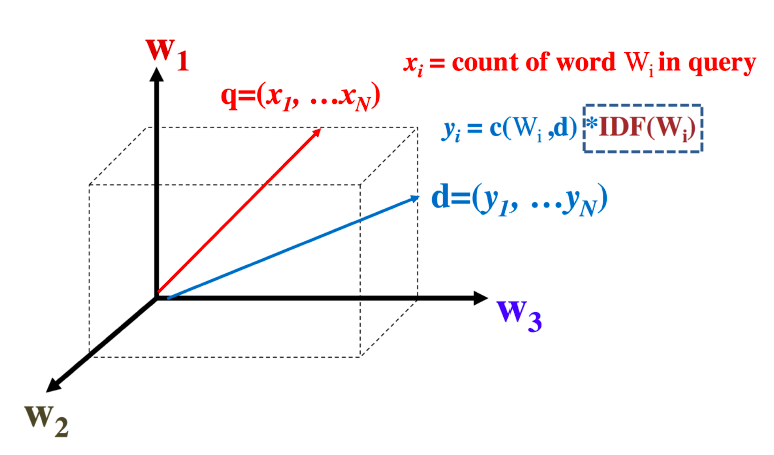
\includegraphics[width=.7\linewidth]{text9}
\end{figure}
\begin{figure}[H]
  \centering
  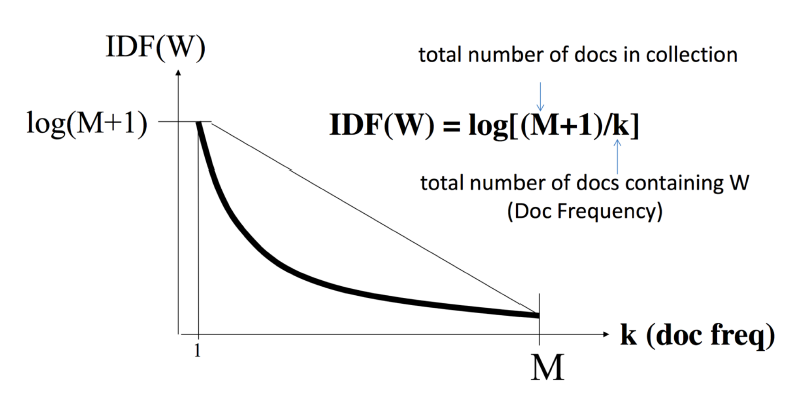
\includegraphics[width=.7\linewidth]{text10}
\end{figure}
In this case "about" which is more common gets penalized wrt to "presidential" , a rarer word.
\begin{figure}[H]
  \centering
  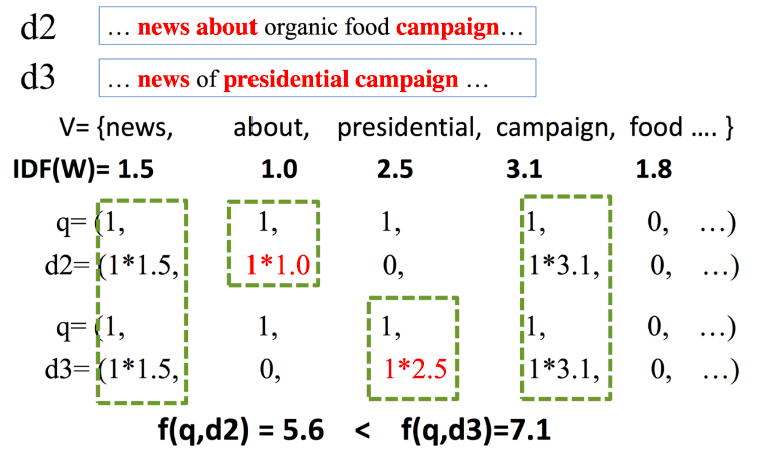
\includegraphics[width=.7\linewidth]{text11}
\end{figure}
The more uncommon a word the higher the IDF score. Usually the denominator uses \textbf{k+1} to avoid 0 occurrence.
Combining TF-IDF:
\begin{figure}[H]
  \centering
  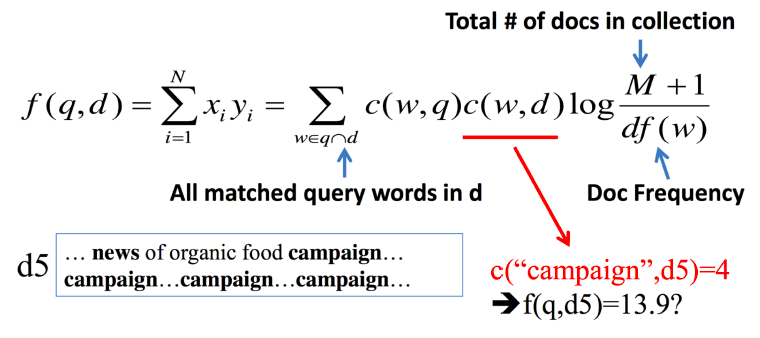
\includegraphics[width=.7\linewidth]{text12}
\end{figure}
The term in red is what causes the last issue: the document d5 has still a score that is too high! It should be rated less , since it contains campaign , which is not common , \textbf{many times} , but the document is actually not so important! This because it appears not often , but then it appears often in \textbf{one document}.

\subsubsection{4.Document Similarity Retrieval : TFTransformations}
This can be solved by two \textbf{transformations} that put an \textbf{upper limit} to the count of term frequency (modifies the count of terms in the document):
\begin{itemize}
\item \textbf{TFTransformation}\\
\begin{figure}[H]
  \centering
  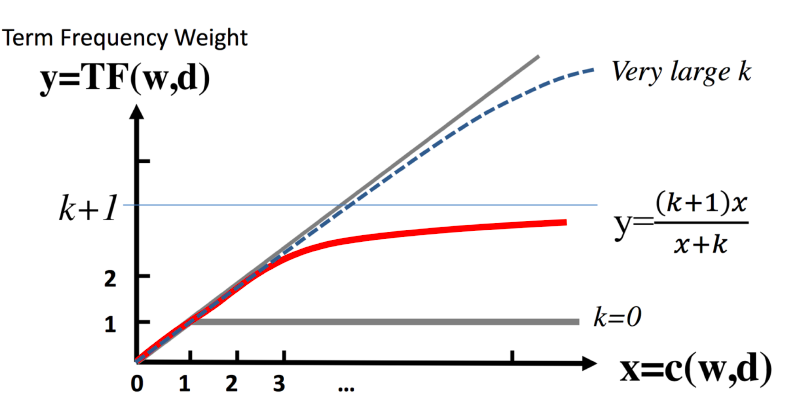
\includegraphics[width=.7\linewidth]{text13}
\end{figure}

\item \textbf{BM25}\\
\begin{figure}[H]
  \centering
  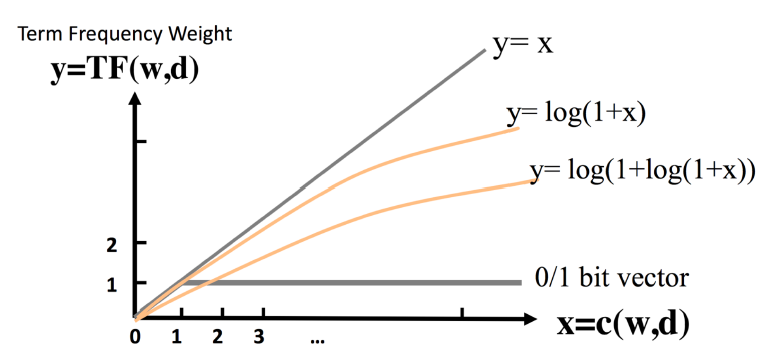
\includegraphics[width=.7\linewidth]{text14}
\end{figure}
\end{itemize}
A final model ,using \textbf{BM25} and \textbf{IDF} to rank documents :
\begin{figure}[H]
  \centering
  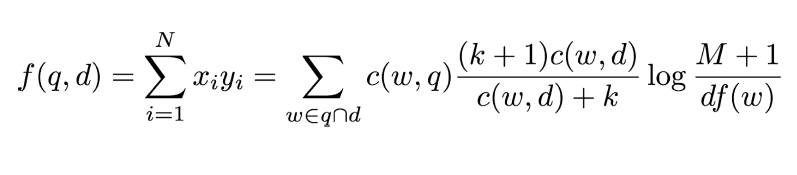
\includegraphics[width=.7\linewidth]{text15}
\end{figure}

\subsubsection{5.Document Similarity Retrieval : Document Length}
Documents need to be \textbf{normalized} in length. This is because longer documents have a better chance of matching the query than shorter ones and thus need to be \textbf{penalized} (avoid \textbf{over-penalization!)}
A document is long because:
\begin{itemize}
\item it has \textbf{more word} $\rightarrow$ should be \textbf{penalized more}
\item it has \textbf{more content} $\rightarrow$ should be \textbf{penalized less}
\end{itemize}
The \textbf{pivoted doc normalizer}:
\begin{itemize}
\item uses \textbf{average} doc length as \textbf{pivot}
\item \textbf{1} if length $|d| = avgdl$
\end{itemize}
\begin{figure}[H]
  \centering
  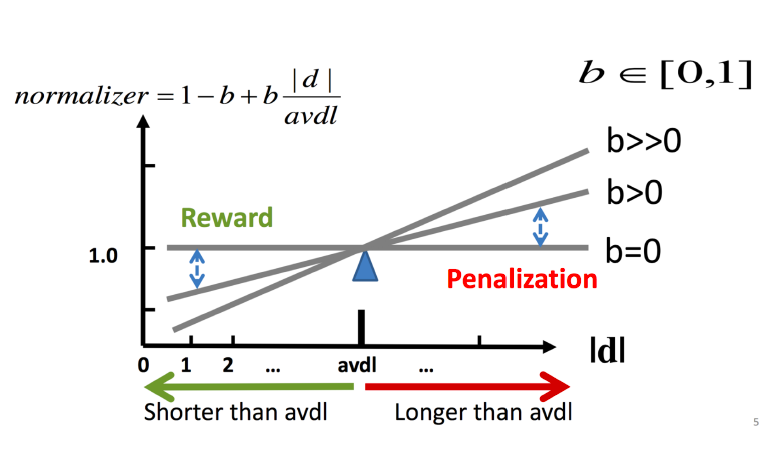
\includegraphics[width=.7\linewidth]{text16}
\end{figure}

\subsubsection{6.Document Similarity Retrieval : State of Art}
\begin{figure}[H]
  \centering
  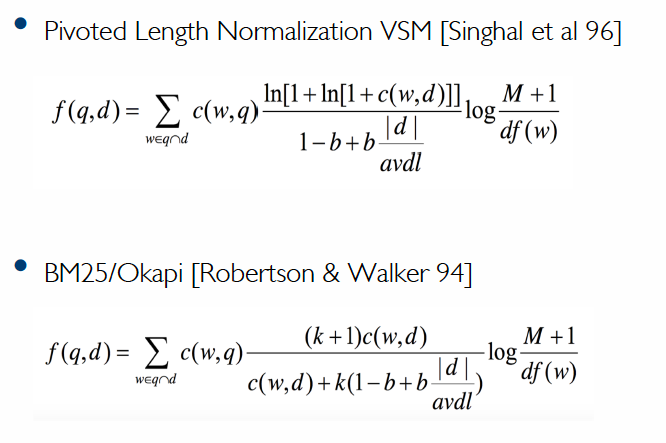
\includegraphics[width=.7\linewidth]{text17}
\end{figure}

\subsection{From text to numerical vectors}
Text is processed using \textbf{tokens} ,and textbf{keywords} are isolated and identified with:
\begin{itemize}
\item  \textbf{Stop word elimination}\\
Stop words are elements that are considered \textbf{uninteresting} wrt to the retrieval and thus eliminated (e.g. : "a" ,"the", "always"...)
\item \textbf{Word Stemming}\\
Different words share \textbf{common prefix} which can replace whole words . E.g.: "computer" , "computing" ,"computerize" are \textbf{replace with} "comput"
\end{itemize}
Another task to deal with is \textbf{dimensionality reduction}.Working on high dimensional space with \textbf{many many keywords}:
\begin{itemize}
\item \textbf{computationally expensive }
\item problems with \textbf{synonymy} and \textbf{polysemy}
\end{itemize}
Dimensionality reduction techniques include :
\begin{itemize}
\item Probabilistic semantic indexing
\item Locality preserving index
\item \textbf{Latent Semantic Indexing}\\
Let $x_i$ be vectors representing documents and X the set of all documents :
$$ \overrightarrow{x_i} ,..., \overrightarrow{x_n} \in R^m \quad X=[\overrightarrow{x_1},...,\overrightarrow{x_n}]$$
Use \textbf{SVD} to reduce the size of frequency table :
 $$ X = U \Sigma V^T$$
 Then approximate $X \approx X_k$ that is obtained from the \textbf{first k vectors of U}.
\end{itemize}

\subsection{Text Classification}
Solves the problem of labeling \textbf{automatically} text documents on the basis of :
\begin{itemize}
\item Topic
\item Style
\item Purpose
\end{itemize}
Usual classification techniques can be used to learn from a training set of \textbf{manually labeled} documents.\\
Features could be : \textbf{keywords}.

\subsubsection{Similarity based text classifiers}
Exploits information retrieval and \textbf{k-nearest neighbour}:
\begin{itemize}
\item for a new document to classify find the \textbf{k} most similar ones
\item documents are classified on the basis of class distribution among the k documents retrieved using \textbf{majority vote}
\item tuning k is \textbf{very important for good results}
\end{itemize}
Limitations are due to \textbf{space overhead} (save documents) and \textbf{time overhead} (retrieve similar documents)

\subsubsection{Dimensionality reduction in text classifiers}
Similar to what is done in VSM to reduce the number of features to represent text : they usually use \textbf{distribution of keywords} among the \textbf{whole database}.\\
In classification also \textbf{correlation } between \textbf{keywords - class label} must be taken into account : rare keywords have a high TF-IDF but might be uniformly distributed among classes.\\
After the dimensionality reduction step a classifier can be applied ( SVM ,Naives Bayes..)

\subsubsection{Example with Naives Bayes Text Classifier}
\begin{itemize}
\item Document categories $\{  C_1, ... ,C_n \}$
\item Document to classify D
\item Probabilistic model $$ P(C_i|D) = \frac{P(D|C_i)P(C_i)}{P(D)}$$
\item Choose class $C^{*}=argmax_c P(C|D) = argmax_C P(D|C)P(C)$
\end{itemize}
Features can be defined as \textbf{words in the document}:
 \begin{figure}[H]
  \centering
  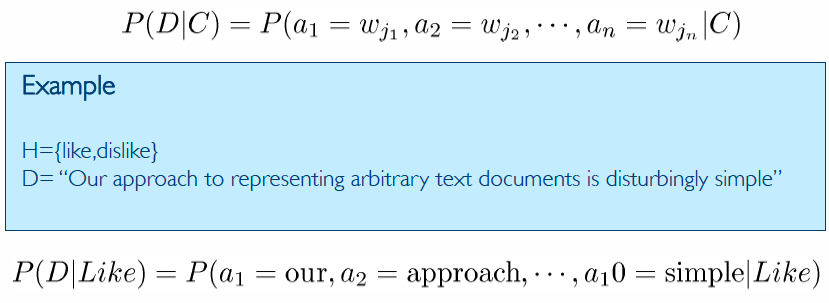
\includegraphics[width=.7\linewidth]{text21}
\end{figure}
 \begin{figure}[H]
  \centering
  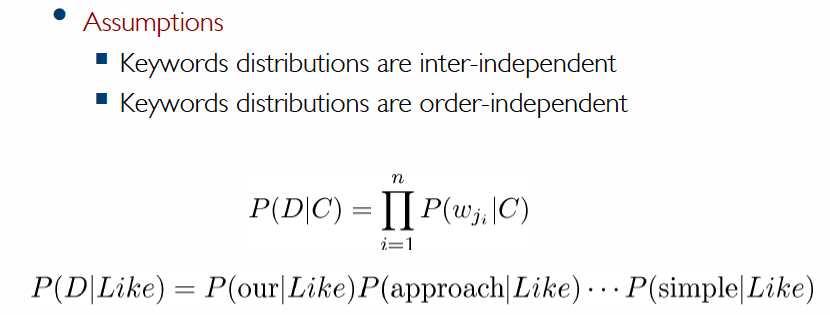
\includegraphics[width=.7\linewidth]{text22}
\end{figure}
 \begin{figure}[H]
  \centering
  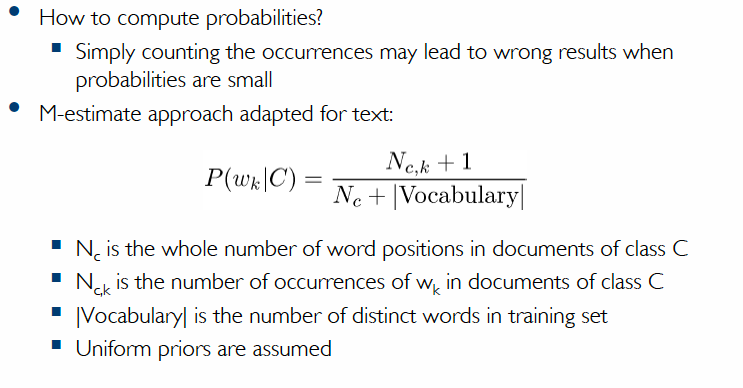
\includegraphics[width=.7\linewidth]{text23}
\end{figure}
 \begin{figure}[H]
  \centering
  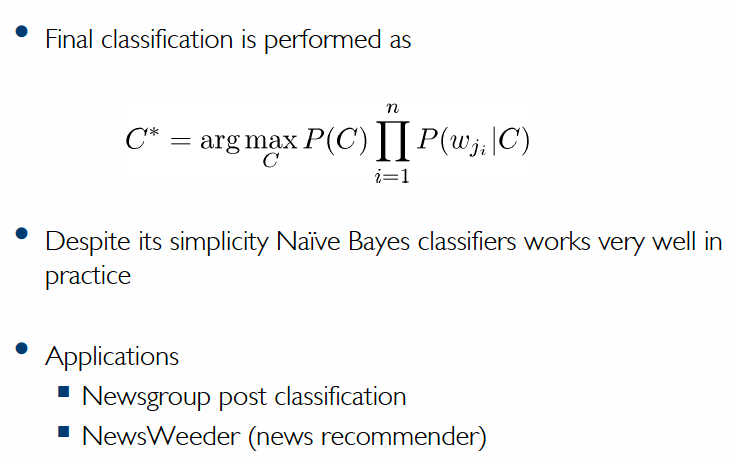
\includegraphics[width=.7\linewidth]{text24}
\end{figure}

\subsection{Word Embeddings}
Learned representation for text where words with \textbf{similar meanings} have \textbf{similar representations}. It a set of methods that represent \textbf{individual words} as \textbf{real-valued vectors} (often up to 10.000 dimensions) in a predefined vector space: each vector is mapped to one vector and the vector values are \textbf{learned} in a way similar to NN.
\\
Words and phrases from the vocabulary are \textbf{mapped}  to vectors of real numbers.
 \begin{figure}[H]
  \centering
  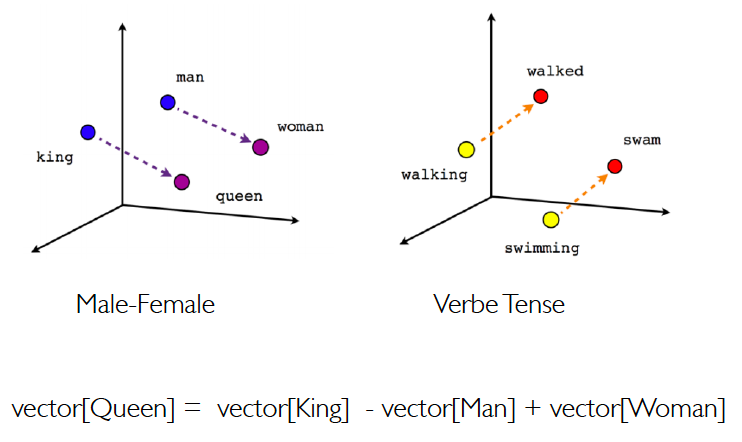
\includegraphics[width=.7\linewidth]{text18}
\end{figure}
This differentiates from the \textbf{word of bags model}:
\begin{itemize}
\item uses \textbf{one hot encoding}
\item \textbf{one bit position} in a huge vector
\item no context information
\end{itemize}
Word Embeddings :
\begin{itemize}
\item each words is a \textbf{point} in continuous space
\item a word is represented by a vector of fixed number of dimensions (generally 300)
\item Generated from a \textbf{huge corpus} using \textbf{unsupervised methods}
\item Dimensions are projections	along different axis 
\end{itemize}
Word embeddings are very useful for :
\begin{itemize}
\item \textbf{word similarity} 
\item\textbf{ machine translation}
\item \textbf{part of speech and name-entity recognition}
\item \textbf{relation extraction}
\item \textbf{sentiment analysis} = usually uses bag of words
\item \textbf{co-reference resolution} = chaining entity mentions across multiple documents :find and unify all contexts where mention occurs?
\item \textbf{clustering} = words in same class occur naturally in similar contexts and have similar embeddings (k-means....)
\item \textbf{Semantic Doc Analysis} = build word distributions for various topics...
\end{itemize}
Word embeddings can be done using :
\begin{itemize}
\item Latent semantic indexing (LSI)
\item Fastext
\item Word2Vec
\end{itemize}

\subsubsection{Word2Vec}
Uses a NN with \textbf{single hidden layer} to ,given a specific word in the middle of a sentence (\textbf{input word} ) predict the \textbf{probability} for every word in our vocabulary of being a \textbf{nearby word} that we chose.\\
The \textbf{hidden layer} is just a \textbf{representation}  of the input word while the output vector is a \textbf{probability distribution}.
 \begin{figure}[H]
  \centering
  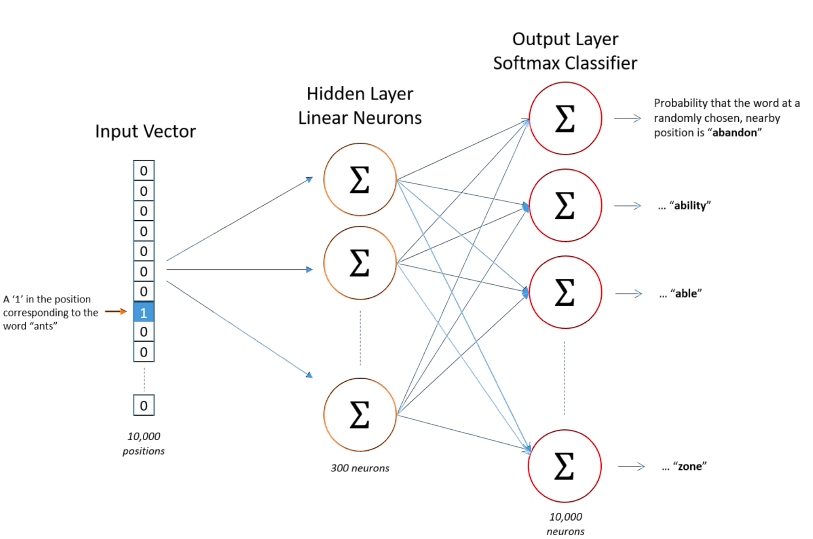
\includegraphics[width=.7\linewidth]{text19}
\end{figure}
 \begin{figure}[H]
  \centering
  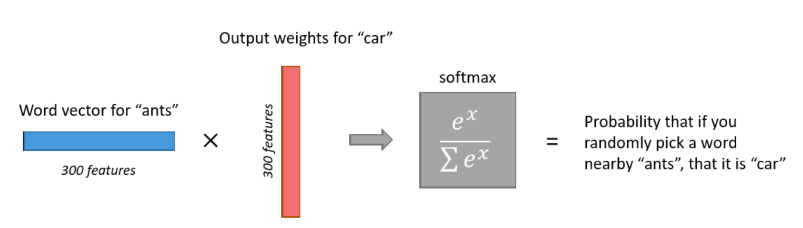
\includegraphics[width=.7\linewidth]{text20}
\end{figure}